\setcounter{chapter}{3}
\chapter{Implementation and Validation of the SOCaaS Platform}
\label{chap:socaas-implementation-validation}

% ========== 4.1 INTRODUCTION ==========
\section{Introduction}
\label{sec:ch4-introduction}

This chapter presents the practical implementation and validation of SOCaaS, an open-source and cloud-native Security Operations Center delivered as a service-oriented platform. The objective is to demonstrate how the conceptual architecture defined in the previous chapter was transformed into a functional environment capable of performing real-time threat detection, automated incident response, alert enrichment, analyst notification, case management, AI-assisted recommendations, and malware analysis through the AI Sandbox. This implementation follows the operational principle that detection, triage, analysis, and response must be connected into a coherent incident handling process rather than treated as isolated technical functions \cite{bejtlich2013nsm,nist-sp800-61r2}.

The implementation was carried out on a Kubernetes cluster deployed in a virtualized laboratory infrastructure. The platform integrates Wazuh as the SIEM layer, a custom Pipeline Gateway as the normalization and enrichment layer, Shuffle as the SOAR engine, TheHive as the case management system, and an AI Sandbox dedicated to suspicious file analysis. These components were not deployed as isolated tools; they were connected into a complete detection and response chain in which endpoint telemetry is collected, normalized, enriched, deduplicated, escalated to analysts, and transformed into investigation cases.

The validation of SOCaaS was performed through controlled attack simulations and malware analysis experiments. The main validation scenario focuses on the AI Sandbox, because it represents a significant added value compared with a traditional SOC pipeline. Instead of only detecting and notifying analysts about a suspicious file, SOCaaS analyzes the file in a temporary isolated VM, extracts indicators of compromise, reconstructs its behavior, maps relevant techniques, and generates an analyst-readable report using DeepSeek-V4-Pro. Additional validation scenarios, including Nmap port scan detection and command-and-control beacon detection, are summarized in this chapter and documented in detail in the appendices.

This chapter therefore has a dual purpose. First, it documents the technical implementation of the SOCaaS platform in a reproducible Kubernetes environment. Second, it evaluates whether the platform can support realistic security operations by reducing alert fatigue, improving investigation context, and shortening the time required to understand suspicious malware behavior.

% ========== 4.2 OVERVIEW OF THE KUBERNETES CLUSTER ==========
\section{Overview of the Kubernetes Cluster}
\label{sec:ch4-cluster-overview}

The SOCaaS platform was deployed in a virtualized environment based on KVM/QEMU with libvirt. The host operating system was Parrot OS, and the virtual machines were connected through the libvirt bridge \texttt{virbr0} using the private network \texttt{192.168.122.0/24}. This environment made it possible to reproduce a small enterprise network while preserving the isolation required for security testing and malware analysis.

The Kubernetes cluster is composed of one control-plane node and two worker nodes. The control-plane node, named \texttt{k8s-master}, is responsible for the Kubernetes API server, scheduling, cluster state coordination, and control operations. The worker node \texttt{k8s-worker1} hosts the SIEM workloads, mainly Wazuh components. The worker node \texttt{k8s-worker2} hosts the SOAR and case management workloads, including Shuffle, Pipeline Gateway, Redis, OpenSearch, TheHive, Cassandra, Elasticsearch, and MinIO. This organization follows the Kubernetes model in which the control plane manages cluster state and worker nodes execute application workloads \cite{k8s-docs,luksa2017kubernetes}.

This separation of workloads was adopted to keep the SIEM processing layer distinct from orchestration and case management services. Wazuh receives and indexes endpoint telemetry, while Shuffle and TheHive perform response automation and investigation management. External access to selected services is provided through HAProxy and Kubernetes NodePort services, allowing dashboards, webhooks, and analyst-facing interfaces to be reached from the laboratory network.

Two monitored endpoints were added to validate SOCaaS detections. The Linux endpoint \texttt{victim-01} was assigned the address \texttt{192.168.122.180}, while the Windows endpoint \texttt{win10-victim} was assigned the address \texttt{192.168.122.98}. These endpoints provide telemetry to Wazuh agents and are used as realistic targets for detection and response scenarios.

\begin{table}[H]
\centering
\caption{SOCaaS Kubernetes Cluster Components}
\label{tab:ch4-cluster-components}
\renewcommand{\arraystretch}{1.35}
\begin{tabularx}{\textwidth}{>{\RaggedRight\arraybackslash}p{3.3cm} >{\RaggedRight\arraybackslash}p{3cm} >{\RaggedRight\arraybackslash}p{3cm} X}
\toprule
\rowcolor{tableheader}
\textbf{Component} & \textbf{Hostname} & \textbf{IP Address} & \textbf{Role in SOCaaS} \\
\midrule
Hypervisor host & Parrot OS host & \texttt{192.168.122.1} & Hosts the KVM/QEMU and libvirt environment and provides the \texttt{virbr0} virtual network. \\
\midrule
Kubernetes control-plane & \texttt{k8s-master} & \texttt{192.168.122.10} & Single Kubernetes control-plane node responsible for cluster control operations. \\
\midrule
Kubernetes worker & \texttt{k8s-worker1} & \texttt{192.168.122.11} & Worker node dedicated to SIEM workloads, mainly Wazuh services. \\
\midrule
Kubernetes worker & \texttt{k8s-worker2} & \texttt{192.168.122.12} & Worker node dedicated to SOAR, Pipeline Gateway, TheHive, and supporting data services. \\
\midrule
Linux victim endpoint & \texttt{victim-01} & \texttt{192.168.122.180} & Linux monitored endpoint used for attack simulation and endpoint telemetry validation. \\
\midrule
Windows victim endpoint & \texttt{win10-victim} & \texttt{192.168.122.98} & Windows monitored endpoint used for Windows security, malware, process, and network event validation. \\
\bottomrule
\end{tabularx}
\end{table}

\begin{figure}[H]
\centering
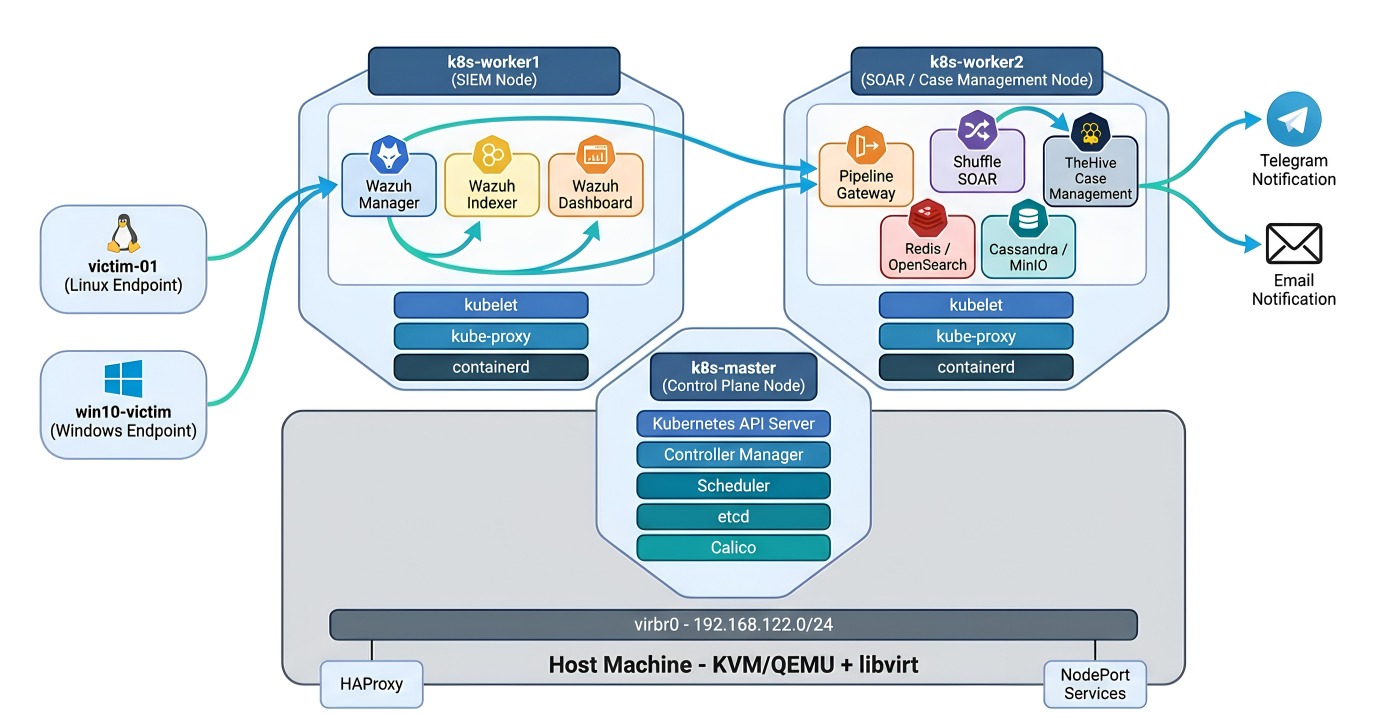
\includegraphics[width=0.82\textwidth]{figs/socaas_kubernetes_cluster_architecture.png}
\caption{SOCaaS Kubernetes Cluster Architecture}
\label{fig:ch4-socaas-kubernetes-cluster}
\end{figure}

The Parrot OS host runs KVM/QEMU and libvirt, with the \texttt{virbr0} network interconnecting the Kubernetes nodes and monitored endpoints. The node \texttt{k8s-worker1} is dedicated to SIEM workloads, while \texttt{k8s-worker2} hosts SOAR, Pipeline Gateway, and TheHive workloads. Linux and Windows victim endpoints appear as monitored systems connected to Wazuh agents.

% ========== 4.3 DEPLOYMENT OF THE KUBERNETES CLUSTER ==========
\section{Deployment of the Kubernetes Cluster}
\label{sec:ch4-kubernetes-deployment}

The Kubernetes cluster was deployed using Kubernetes version \texttt{v1.30.14}. The selected container runtime was \texttt{containerd 2.2.1}, and the cluster networking layer was implemented using Calico \texttt{v3.28.5}. Helm was later used as the package manager for SOCaaS components. This combination provided a stable foundation for hosting containerized security tools while keeping the deployment close to production Kubernetes practices \cite{kubernetes-container-runtimes,containerd-docs,calico-docs}.

The first implementation step consisted of installing and configuring \texttt{containerd} on all Kubernetes nodes. The runtime was configured before installing Kubernetes components because every pod scheduled by Kubernetes depends on a functional container runtime. Afterward, the packages \texttt{kubeadm}, \texttt{kubelet}, and \texttt{kubectl} were installed on the control-plane and worker nodes. The \texttt{kubelet} service manages pod execution on each node, \texttt{kubeadm} provides the initialization and joining workflow, and \texttt{kubectl} provides the administrative interface used to verify and manage the cluster \cite{kubeadm-install}.

The control-plane was initialized on \texttt{k8s-master} using \texttt{kubeadm init}. This operation created the Kubernetes API server, controller manager, scheduler, and required cluster state configuration. After the control-plane became available, Calico was deployed to provide pod-to-pod networking across the cluster. Calico was selected because it is a mature Kubernetes CNI and supports network policy capabilities, which are important for future hardening of SOCaaS communications.

The worker nodes \texttt{k8s-worker1} and \texttt{k8s-worker2} were then joined to the cluster using the join command produced by the control-plane initialization process. The cluster status was verified after the join operation to ensure that all nodes reached the \texttt{Ready} state and that Calico pods were running correctly. Detailed terminal commands and full installation evidence are preserved in the implementation evidence appendix when required.

\begin{figure}[H]
\centering
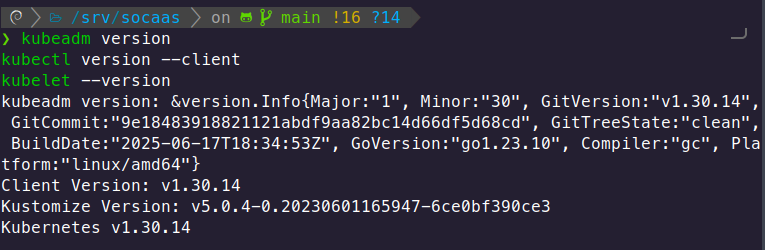
\includegraphics[width=0.92\textwidth]{figs/kubernetes_packages_installed.png}
\caption{Installed Kubernetes Packages and Versions}
\label{fig:ch4-kubernetes-packages}
\end{figure}

The package version evidence confirms that \texttt{kubeadm}, \texttt{kubelet}, and \texttt{kubectl} were installed and available for the cluster deployment workflow.

\begin{figure}[H]
\centering
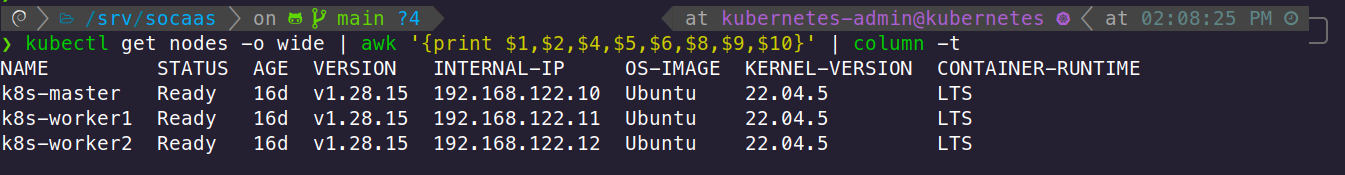
\includegraphics[width=0.82\textwidth]{figs/kubectl_get_nodes.png}
\caption{Kubernetes Cluster Status}
\label{fig:ch4-cluster-status}
\end{figure}

All three nodes are in the \texttt{Ready} state with containerd as the container runtime. Node internal IP addresses are \texttt{192.168.122.10} (master), \texttt{192.168.122.11} (worker1), and \texttt{192.168.122.12} (worker2).

% ========== 4.4 DEPLOYMENT OF SOCAAS SECURITY TOOLS ==========
\section{Deployment of SOCaaS Security Tools}
\label{sec:ch4-tools-deployment}

The SOCaaS security tools were deployed on Kubernetes through manifests and Helm packaging. Namespaces were used to organize the platform according to functional areas. The namespace \texttt{socaas-system} stores Helm release state, \texttt{socaas-siem} contains the Wazuh SIEM deployment, \texttt{socaas-soar} contains Shuffle, Pipeline Gateway, Redis, and OpenSearch, and \texttt{socaas-thehive} contains TheHive, Cassandra, MinIO, and Elasticsearch.

This namespace separation improves operational clarity. It allows SIEM, SOAR, and case management resources to be inspected independently while preserving the integration between them through Kubernetes services and webhooks. It also prepares the platform for future hardening, where network policies and role-based access controls can be applied by namespace.

\subsection{Wazuh SIEM Deployment}
\label{subsec:ch4-wazuh-deployment}

Wazuh was deployed as the SIEM layer of SOCaaS in the \texttt{socaas-siem} namespace. The deployed components include Wazuh Manager \texttt{4.8.2}, Wazuh Indexer \texttt{4.8.2}, and Wazuh Dashboard \texttt{4.8.2}. These workloads were placed on \texttt{k8s-worker1}, which was dedicated to SIEM processing in order to separate detection and indexing activities from SOAR and case management workloads \cite{wazuh-server,wazuh-indexer,wazuh-dashboard}.

The Wazuh Manager receives endpoint telemetry from agents installed on the monitored Linux and Windows machines. The Linux agent was installed on \texttt{victim-01}, and the Windows agent was installed on \texttt{win10-victim}. These agents collect file integrity events, operating system events, Windows Defender alerts, process activity, and network-related telemetry. The Wazuh Dashboard provides the analyst-facing visualization interface, while the Wazuh Indexer stores indexed security events and alerts. This design reflects the central role of log collection, indexing, correlation, and review in security monitoring \cite{chuvakin2012logging,wazuh-agent}.

Custom Wazuh rules were added to support SOCaaS validation scenarios. These rules include UFW and port scan detection, File Integrity Monitoring malware detection, Windows Defender malware detection, and Windows process and network event detection. Their role is to convert raw endpoint activity into structured alerts that can be consumed by the automation pipeline.

To connect Wazuh with the SOCaaS automation layer, a Wazuh Alert Forwarder sidecar was implemented. This sidecar forwards Wazuh alerts to the Pipeline Gateway instead of sending raw alerts directly to Shuffle. This design gives SOCaaS a controlled integration point where alerts can be validated, normalized, enriched, and deduplicated before entering the SOAR workflow.

\begin{figure}[H]
\centering
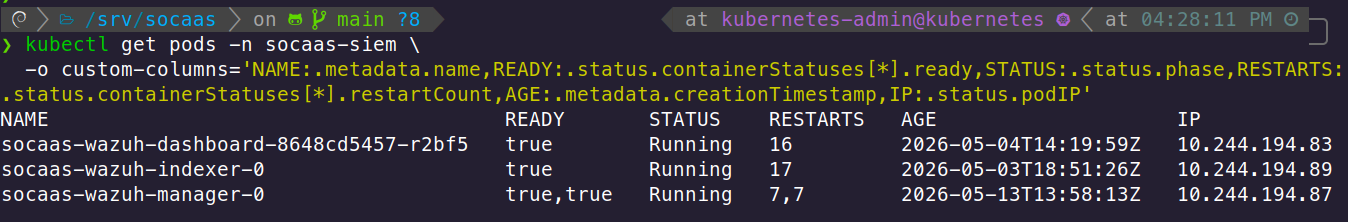
\includegraphics[width=0.82\textwidth]{figs/wazuh_pods.png}
\caption{Wazuh Pods Running}
\label{fig:ch4-wazuh-pods}
\end{figure}

The Wazuh Dashboard, Wazuh Indexer, and Wazuh Manager pods are in the \texttt{Running} state with their respective readiness counts, restart counts, and pod IP addresses allocated on the Calico network.

\begin{figure}[H]
\centering
\begin{adjustbox}{center}
  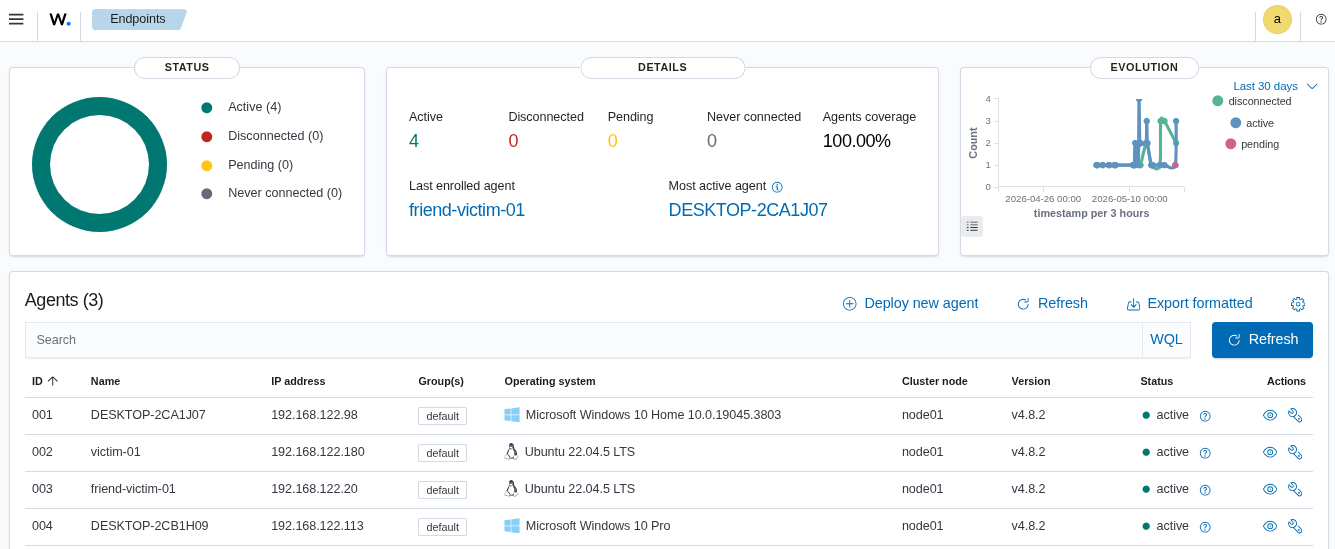
\includegraphics[width=1.2\textwidth]{figs/wazuh_dashboard_agents.png}
\end{adjustbox}
\caption{Wazuh Dashboard -- Endpoints}
\label{fig:ch4-wazuh-dashboard}
\end{figure}


\begin{figure}[H]
\centering
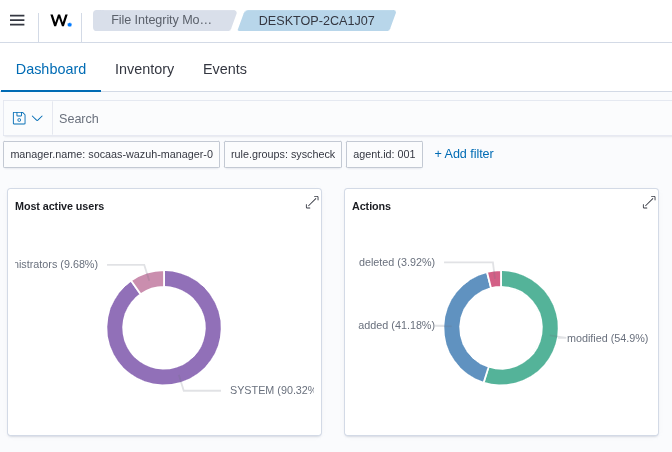
\includegraphics[width=0.82\textwidth]{figs/wazuh_deleted_files_fim_dashboard.png}
\caption{Wazuh File Integrity Monitoring Alerts}
\label{fig:ch4-wazuh-alerts}
\end{figure}

The FIM dashboard displays syscheck alerts for agent 001 (\texttt{DESKTOP-2CA1J07}), showing file actions including deletion, modification, and addition events detected during the validation scenarios.

\subsection{Pipeline Gateway Deployment}
\label{subsec:ch4-pipeline-gateway}

The Pipeline Gateway is a custom integration service implemented with Python \texttt{3.12}. It acts as the controlled bridge between Wazuh, Shuffle SOAR, and TheHive. Wazuh alerts are sent by the Alert Forwarder to the Pipeline Gateway endpoint \texttt{/hooks/wazuh}. Each incoming request is validated using a webhook secret so that unauthorized systems cannot inject alerts into the automation pipeline.

After validation, the Pipeline Gateway extracts observables from the Wazuh alert. These observables include IP addresses, domains, hashes, URLs, ports, and process names. The extracted values are transformed into a normalized alert structure before any AI-assisted processing is performed. This is an important design decision, because deterministic parsing ensures that downstream automation receives explicit evidence rather than inferred or hallucinated indicators.

The gateway also performs VirusTotal enrichment where applicable. Public IP addresses, domains, hashes, and URLs can be enriched to add reputation and threat intelligence context to the alert. Private laboratory addresses, such as those in \texttt{192.168.122.0/24}, are handled with caution because they cannot be meaningfully scored by public reputation services \cite{virustotal-api-v3}.

Alert deduplication is implemented using a 300-second TTL cache. During noisy activity, such as port scanning, Wazuh may generate several alerts that represent the same operational incident. The deduplication mechanism reduces repeated alerts before they reach Shuffle and TheHive, helping analysts focus on actionable cases rather than duplicate notifications.

The resulting data flow is Wazuh alert, Alert Forwarder, Pipeline Gateway, deduplication, VirusTotal enrichment, Shuffle workflow, and TheHive context creation. The Pipeline Gateway therefore provides both security control and operational quality control for the SOCaaS pipeline.

\begin{figure}[H]
\centering
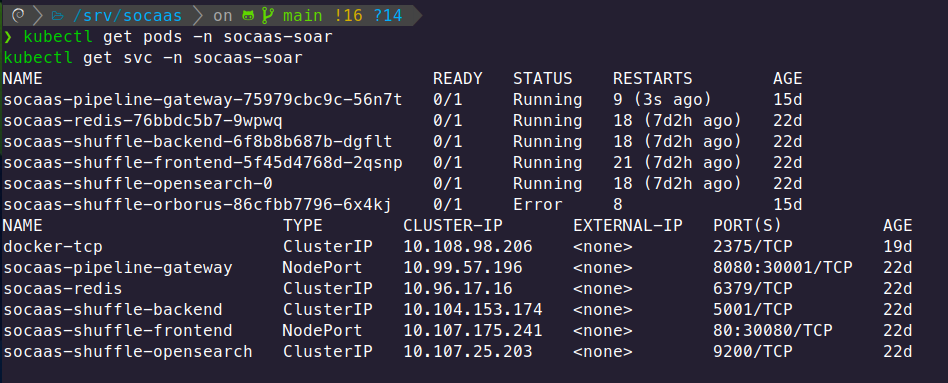
\includegraphics[width=0.95\textwidth]{figs/pipeline_gateway_pod_service.png}
\caption{Pipeline Gateway Pod and Kubernetes Service}
\label{fig:ch4-pipeline-pod-service}
\end{figure}

The Kubernetes service evidence shows that the Pipeline Gateway is exposed in the \texttt{socaas-soar} namespace through a NodePort service on port \texttt{30001}. The screenshot is used as deployment and service-exposure evidence; pod readiness shown in this terminal view should not be interpreted as a full health validation of all SOAR components.

\subsection{Shuffle SOAR Deployment}
\label{subsec:ch4-shuffle-deployment}

Shuffle was deployed in the \texttt{socaas-soar} namespace as the SOAR component of SOCaaS. The deployment includes Shuffle Frontend, Shuffle Backend, Orborus, Redis, and OpenSearch. Shuffle receives normalized alerts from the Pipeline Gateway and executes the automation workflow responsible for triage, enrichment, notification, and case creation \cite{shuffle-docs,shuffle-arch}.

The implemented workflow is named \texttt{SOCaaS Wazuh Alert Triage}. It begins with a webhook trigger and proceeds through alert normalization, threat intelligence enrichment, AI-assisted recommendation generation, notification construction, and TheHive case creation. The workflow was designed to keep the analyst informed while also preserving detailed evidence inside TheHive.

\begin{table}[H]
\centering
\small
\caption{SOCaaS Wazuh Alert Triage Workflow}
\label{tab:ch4-shuffle-workflow}
\renewcommand{\arraystretch}{1.35}

\begin{tabularx}{\textwidth}{
>{\centering\arraybackslash}p{0.9cm}
>{\RaggedRight\arraybackslash}p{3.6cm}
>{\RaggedRight\arraybackslash}X
}
\toprule
\rowcolor{tableheader}
\textbf{Step} & \textbf{Workflow Action} & \textbf{Operational Purpose} \\
\midrule

1 & Webhook Reception
& Receives the normalized alert sent by the Pipeline Gateway. \\

\midrule
2 & Alert Normalization
& Confirms that alert fields are consistently structured before enrichment and notification. \\

\midrule
3 & Threat Intelligence Enrichment
& Enriches extracted observables with external reputation and threat intelligence where applicable. \\

\midrule
4 & AI Recommendation Generation
& Produces analyst-oriented response recommendations from structured alert context. \\

\midrule
5 & Investigation Context Building
& Builds the investigation narrative used for TheHive cases and email notifications. \\

\midrule
6 & Telegram Notification
& Sends a short alert to analysts for rapid awareness. \\

\midrule
7 & Email Notification
& Sends a richer notification containing evidence and recommended actions. \\

\midrule
8 & TheHive Case Creation
& Creates a formal case in TheHive with observables and triage context. \\

\midrule
9 & Final Response
& Returns the workflow execution status after automation is completed. \\

\bottomrule
\end{tabularx}
\end{table}

Telegram was intentionally limited to short alerts because mobile notifications should provide immediate awareness without overwhelming the analyst. TheHive and email receive richer context, including observables, enrichment results, and AI-assisted recommendations, because these channels are better suited to formal investigation.

\begin{figure}[H]
\centering
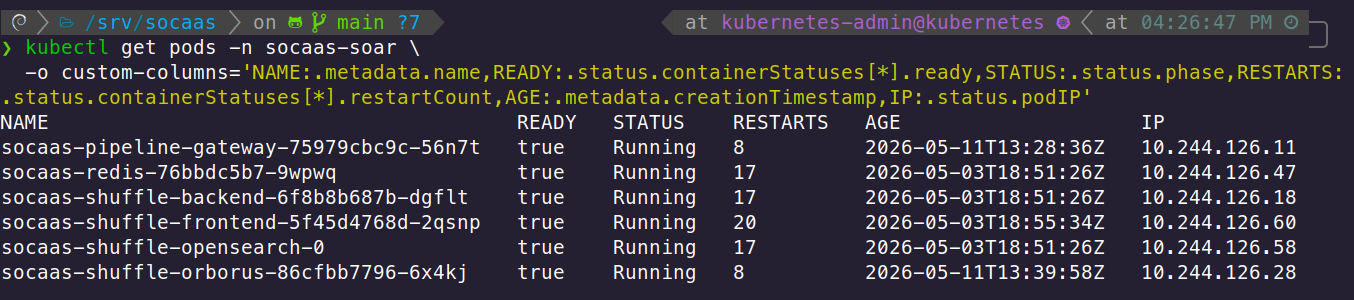
\includegraphics[width=0.82\textwidth]{figs/shuffle_pods_pipeline_gateway.png}
\caption{Shuffle Pods Running}
\label{fig:ch4-shuffle-pods}
\end{figure}

The Shuffle Frontend, Backend, Orborus, Redis, OpenSearch, and Pipeline Gateway pods are operational in the \texttt{socaas-soar} namespace, confirming that the SOAR layer is correctly deployed.

\begin{figure}[H]
\centering
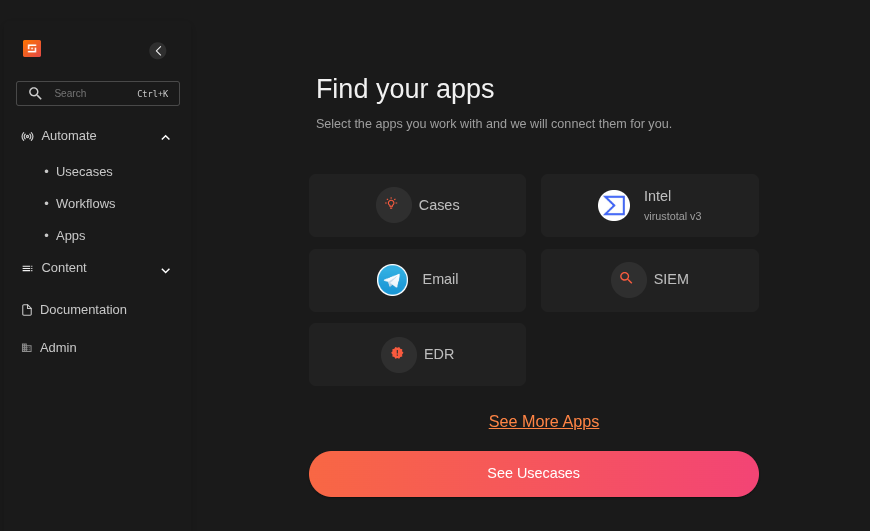
\includegraphics[width=0.82\textwidth]{figs/shuffle_welcome_dashboard.png}
\caption{Shuffle Dashboard and Application Workspace}
\label{fig:ch4-shuffle-dashboard}
\end{figure}

The Shuffle workspace provides the analyst and administrator interface for managing applications, workflows, and automation executions used by SOCaaS.

\begin{figure}[H]
\centering
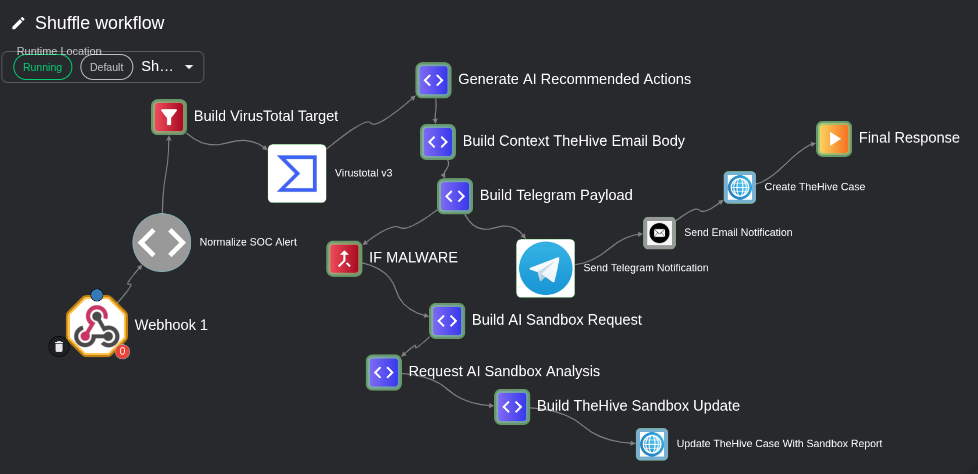
\includegraphics[width=0.82\textwidth]{figs/shuffle_final_workflow_canvas.png}
\caption{Shuffle Workflow Canvas}
\label{fig:ch4-shuffle-workflow-canvas}
\end{figure}

The complete Shuffle workflow showing the webhook trigger, alert normalization, VirusTotal enrichment, AI recommended actions, Telegram and email payload construction, TheHive case creation, malware branch, AI Sandbox request, and final response node.

\begin{figure}[H]
\centering
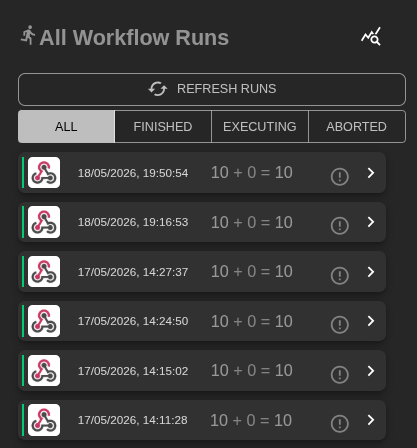
\includegraphics[width=0.58\textwidth]{figs/shuffle_workflow_runs_new.png}
\caption{Shuffle Workflow Runs Showing Successful SOCaaS Executions}
\label{fig:ch4-shuffle-execution}
\end{figure}

The workflow run evidence confirms that SOCaaS automation executions completed successfully after alerts were received and processed by Shuffle.

\subsection{TheHive Case Management Deployment}
\label{subsec:ch4-thehive-deployment}

TheHive was deployed in the \texttt{socaas-thehive} namespace as the case management component of SOCaaS. The deployed version is TheHive \texttt{5.3.11-1}. TheHive provides the investigation interface where alerts are transformed into cases, observables, tasks, and evidence records \cite{thehive-docs,thehive5-kubernetes}.

TheHive was deployed with Cassandra, Elasticsearch \texttt{7.10.2}, and MinIO. Cassandra stores the primary case data and therefore represents the main database backend for TheHive. Elasticsearch is used as the search index, enabling efficient querying and retrieval of investigation records. MinIO is used as object and file storage for attachments, artifacts, and generated reports. This backend separation is consistent with TheHive documentation, which distinguishes database storage, search indexing, and file storage responsibilities \cite{thehive5-requirements,thehive5-db-index}.

The organization configured for this implementation is \texttt{socaas}. The integration user used by Shuffle is \texttt{socaas-shuffle@thehive.local}. API calls to TheHive require the header \texttt{X-Organisation: socaas}, which ensures that case creation and observable updates are executed in the correct organizational context.

In the SOCaaS pipeline, TheHive receives enriched alert context from Shuffle. A created case can include the alert summary, extracted observables, VirusTotal enrichment results, AI-assisted analyst recommendations, and references to AI Sandbox reports. This gives the analyst a centralized investigation space instead of forcing them to reconstruct the incident from disconnected tool outputs.

\begin{figure}[H]
\centering
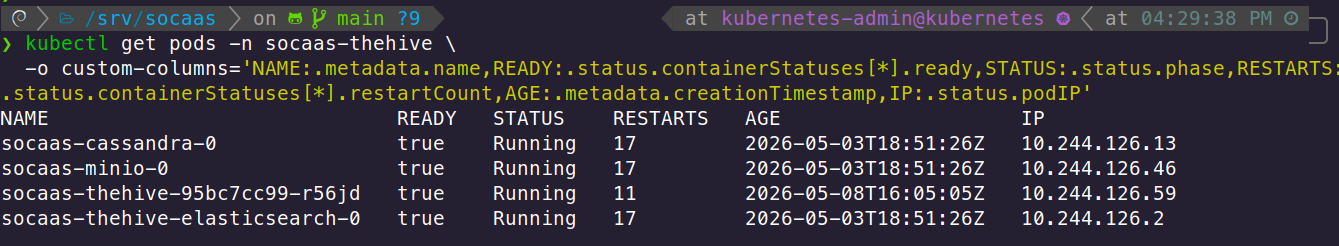
\includegraphics[width=0.82\textwidth]{figs/thehive_pods.png}
\caption{TheHive Pods Running}
\label{fig:ch4-thehive-pods}
\end{figure}

Cassandra, MinIO, TheHive, and Elasticsearch pods are in the \texttt{Running} state with pod IP addresses assigned, confirming that the case management backend is operational.

\begin{figure}[H]
\centering
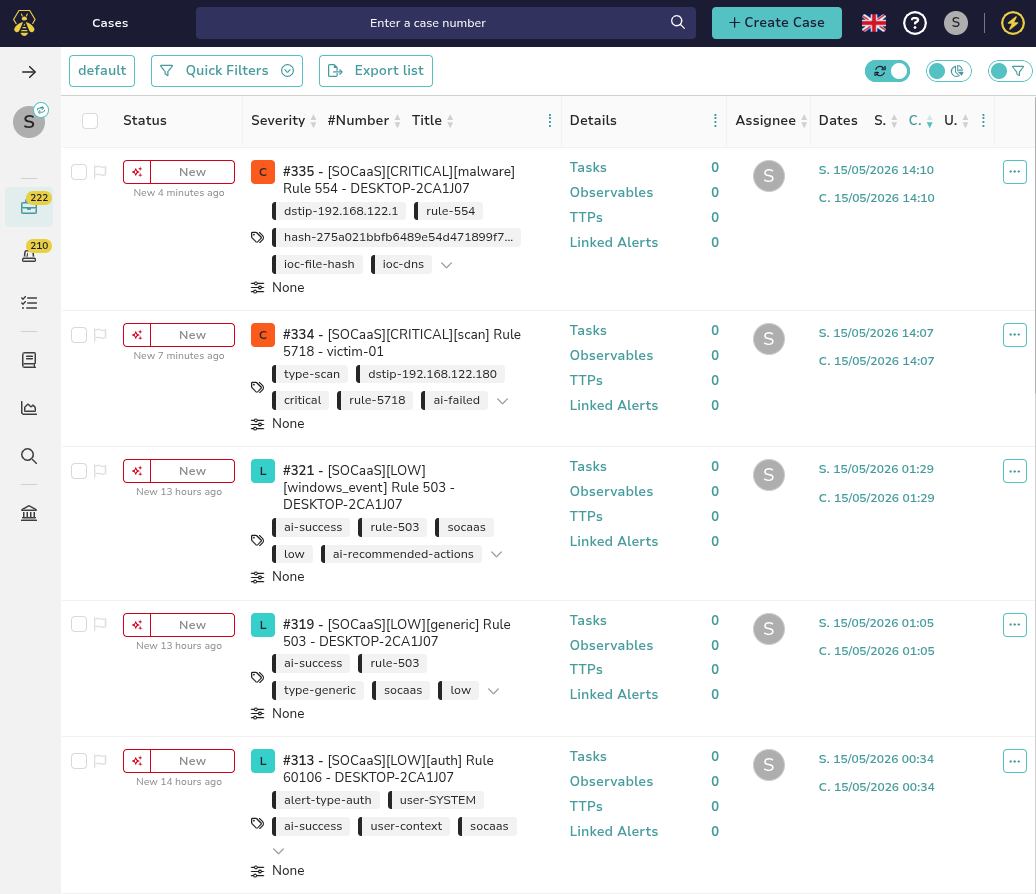
\includegraphics[width=0.82\textwidth]{figs/thehive_cases_dashboard.png}
\caption{TheHive Cases Dashboard}
\label{fig:ch4-thehive-dashboard}
\end{figure}

The dashboard shows multiple SOCaaS cases created by the automation pipeline, including CRITICAL malware and scan cases with associated severity, tags, tasks, observables, TTPs, and linked alerts.

\begin{figure}[H]
\centering
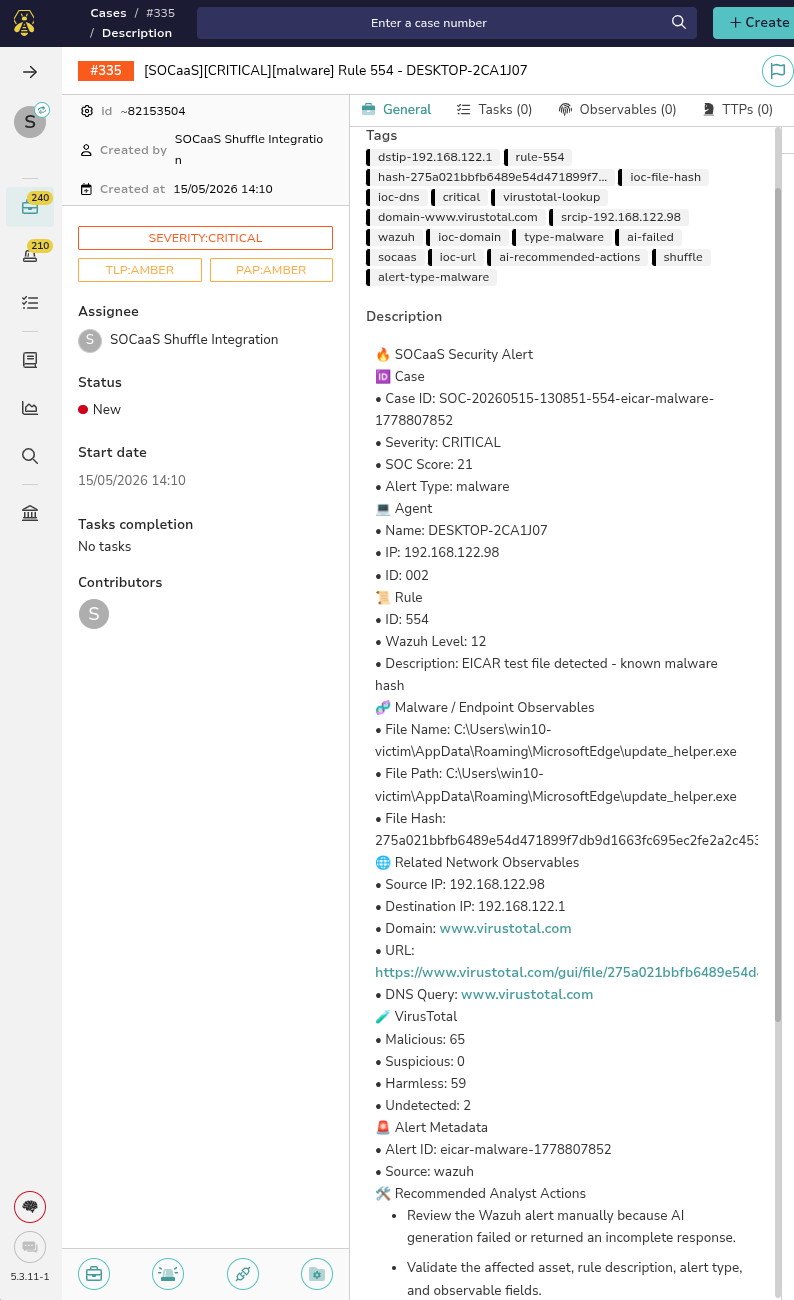
\includegraphics[width=0.82\textwidth]{figs/thehive_malware_case_detail.png}
\caption{Created TheHive Case}
\label{fig:ch4-created-thehive-case}
\end{figure}

A CRITICAL malware case automatically created by the SOCaaS workflow, showing the case ID \texttt{SOC-20260515-130851-554}, severity, SOC score of 21, agent details, Wazuh rule 554 for EICAR test file detection, malware file path and hash, network observables, VirusTotal results (65 malicious), and AI-recommended analyst actions.

% ========== 4.5 IMPLEMENTATION OF THE SOCAAS HELM CHART ==========
\section{Implementation of the SOCaaS Helm Chart}
\label{sec:ch4-helm-chart}

The SOCaaS deployment was packaged as a Helm chart named \texttt{socaas}. Helm was used because the platform consists of multiple Kubernetes objects distributed across several namespaces, including Deployments, Services, ConfigMaps, storage definitions, environment configuration, and integration endpoints. Managing these resources manually would make the deployment harder to reproduce and more error-prone \cite{helm-docs}.

The Helm chart provides repeatability. A SOCaaS deployment can be installed, upgraded, or removed through a controlled release process instead of applying individual manifests manually. This is important for a SOCaaS model because the platform is intended to be reusable for different client environments. Helm also makes the project easier to maintain because manifests can be grouped by component and parameterized through values.

The chart structure groups templates according to platform function. SIEM templates define Wazuh-related resources, SOAR templates define Shuffle and Pipeline Gateway resources, and TheHive templates define TheHive and its supporting services. The namespace \texttt{socaas-system} stores Helm release state, which helps track the deployed version and operational status of the platform.

\begin{figure}[H]
\centering
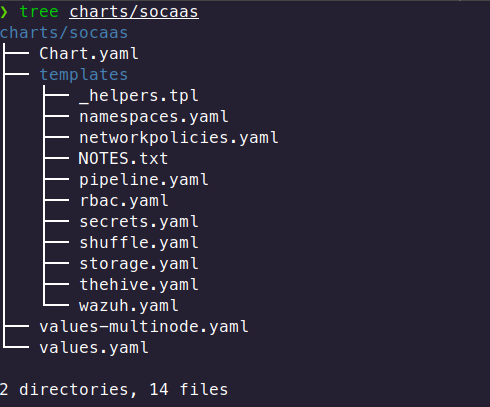
\includegraphics[width=0.62\textwidth]{figs/helm_chart_structure_tree.png}
\caption{SOCaaS Helm Chart Directory Structure}
\label{fig:ch4-helm-chart-structure}
\end{figure}

The chart directory groups deployment values, metadata, templates, and generated chart artifacts in a structure suitable for repeatable SOCaaS installation.

\begin{figure}[H]
\centering
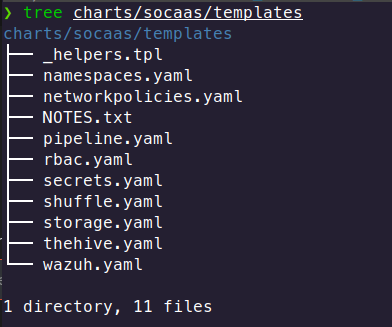
\includegraphics[width=0.60\textwidth]{figs/helm_templates_folder.png}
\caption{SOCaaS Helm Templates Folder}
\label{fig:ch4-helm-templates}
\end{figure}

The templates folder contains the Kubernetes manifests used to deploy namespaces, network policies, Pipeline Gateway, Shuffle, TheHive, Wazuh, and supporting services.

\begin{figure}[H]
\centering
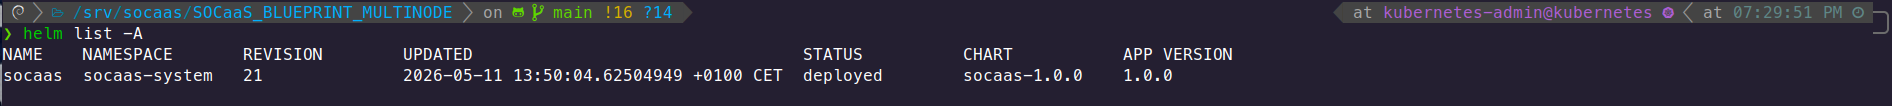
\includegraphics[width=0.98\textwidth]{figs/helm_deployment_success.png}
\caption{Successful SOCaaS Helm Deployment}
\label{fig:ch4-helm-deployment}
\end{figure}

The Helm deployment output confirms that the \texttt{socaas} chart was installed successfully, providing evidence that the platform can be deployed as a reusable Kubernetes package.

% ========== 4.6 END-TO-END DETECTION AND RESPONSE PIPELINE ==========
\section{End-to-End Detection and Response Pipeline}
\label{sec:ch4-end-to-end-pipeline}

The implemented SOCaaS pipeline connects endpoint activity to automated triage and case management. The flow begins when an attacker action, malware execution, reconnaissance scan, or suspicious network communication occurs on a monitored endpoint. The Wazuh agent installed on the endpoint collects telemetry and forwards it to the Wazuh Manager. This chain reflects established network security monitoring and incident response practice, where collection, detection, triage, and response must be traceable from evidence to action \cite{bejtlich2013nsm,nist-sp800-61r2}.

The Wazuh Manager evaluates the event using built-in and custom detection rules. When an alert is produced, it is made available to the Alert Forwarder sidecar, which sends it to the Pipeline Gateway. The Pipeline Gateway validates the request, extracts observables, normalizes the alert, performs enrichment, and applies deduplication using its 300-second TTL cache.

After this processing stage, the normalized alert is sent to Shuffle SOAR. Shuffle executes the \texttt{SOCaaS Wazuh Alert Triage} workflow, enriches the alert further, generates AI-assisted recommendations, sends notifications, and creates a case in TheHive. Telegram is used for short analyst alerts, while email and TheHive contain richer investigation context. When a suspicious file is involved, the AI Sandbox can be invoked to analyze the file and generate a malware analysis report.

The operational flow can be summarized as follows: attacker activity, malware execution, or scan \(\rightarrow\) victim endpoint \(\rightarrow\) Wazuh agent \(\rightarrow\) Wazuh Manager \(\rightarrow\) Wazuh alerts \(\rightarrow\) Alert Forwarder \(\rightarrow\) Pipeline Gateway \(\rightarrow\) Shuffle SOAR \(\rightarrow\) Telegram and email notification \(\rightarrow\) TheHive case \(\rightarrow\) optional AI Sandbox analysis.

\begin{figure}[H]
\centering
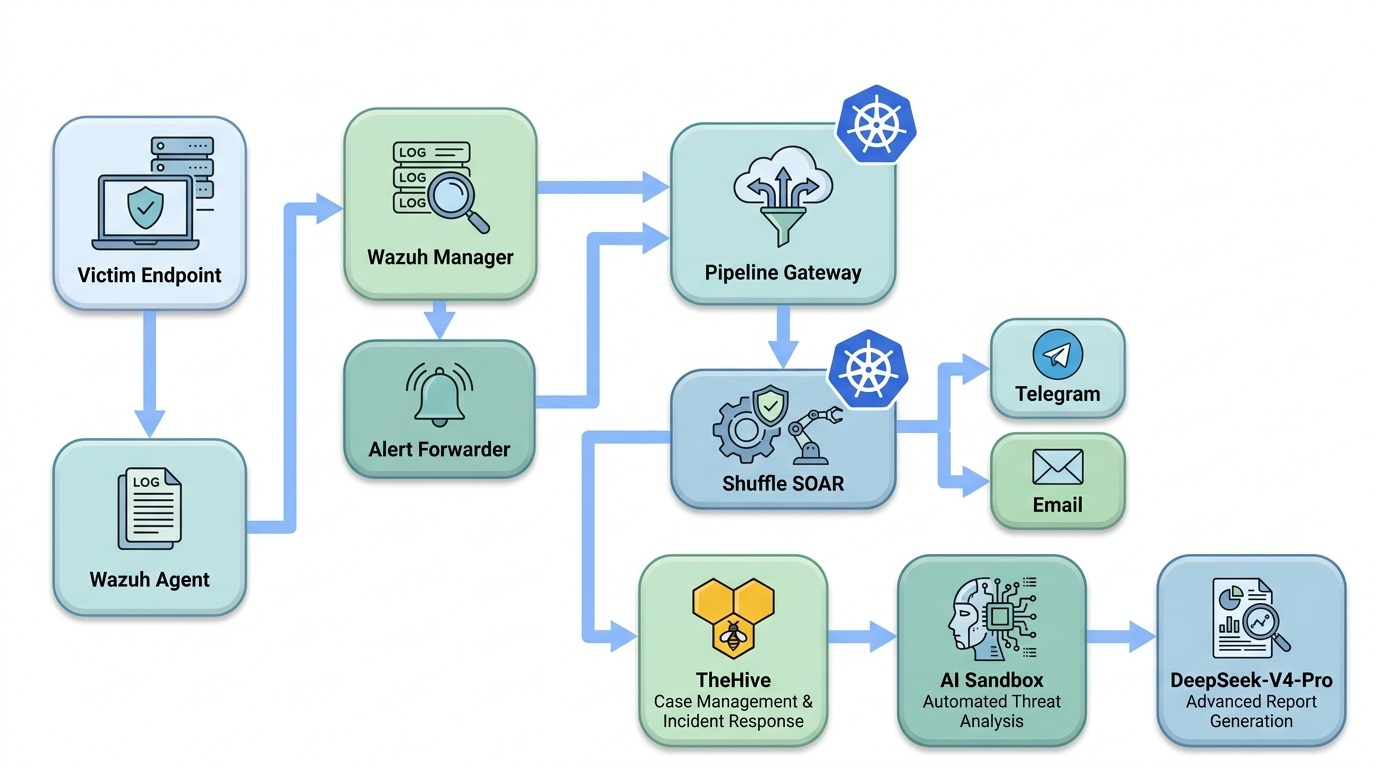
\includegraphics[width=0.92\textwidth]{figs/socaas_end_to_end_pipeline_diagram.jpg}
\caption{End-to-End SOCaaS Detection and Response Pipeline}
\label{fig:ch4-end-to-end-pipeline}
\end{figure}

The pipeline diagram summarizes the implemented SOCaaS flow from endpoint detection to Wazuh, Pipeline Gateway normalization, Shuffle SOAR automation, analyst notification, TheHive case management, and optional AI Sandbox analysis.

% ========== 4.7 AI-ASSISTED ALERT TRIAGE ==========
\section{AI-Assisted Alert Triage}
\label{sec:ch4-ai-triage}

AI-assisted alert triage was implemented to improve the quality and speed of analyst decision-making. The AI recommendation node in the Shuffle workflow receives normalized structured alert context and produces recommended actions, concise evidence summaries, and response guidance. The output is designed to support containment, investigation, escalation, and evidence preservation decisions, which are core activities in incident handling guidance \cite{nist-sp800-61r2}.

The AI component is treated as an assistant rather than as a final decision-maker. Deterministic parsing and normalization are performed before the AI step. This guardrail is essential because the AI must not invent observables or create evidence that was not extracted from the alert. IP addresses, domains, hashes, URLs, ports, and process names are extracted by the Pipeline Gateway before the alert reaches the recommendation node.

The AI output is used mainly to enrich TheHive and email context. TheHive receives the full explanation because it is the formal investigation workspace. Email receives a detailed analyst-oriented summary. Telegram remains short and only carries the information necessary for immediate awareness. This separation of notification channels prevents mobile alert overload while preserving complete context for the investigation record.

The practical benefit of the AI-assisted triage layer is that analysts do not begin with raw logs only. They receive a structured interpretation of the alert, suggested containment steps, and a clear starting point for investigation. However, analyst validation remains mandatory before high-impact response actions are performed.

\begin{figure}[H]
\centering
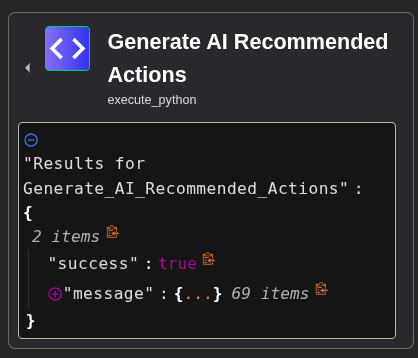
\includegraphics[width=0.55\textwidth]{figs/shuffle_generate_ai_recommended_actions_node.png}
\caption{Shuffle AI Recommended Actions Node Output}
\label{fig:ch4-shuffle-ai-recommendations-node}
\end{figure}

The Shuffle node output illustrates how structured alert context is converted into recommended actions during workflow execution.

\begin{figure}[H]
\centering
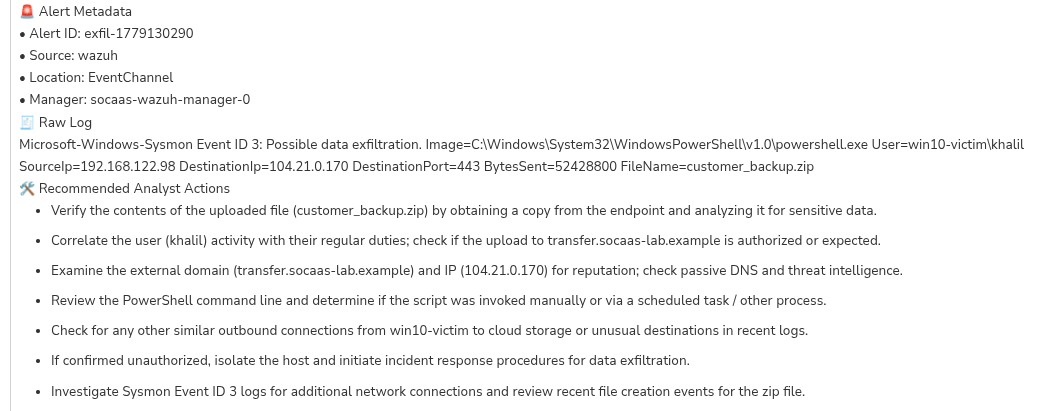
\includegraphics[width=0.95\textwidth]{figs/ai_recommendations_data_exfiltration.png}
\caption{AI Recommended Analyst Actions for Data Exfiltration Alert}
\label{fig:ch4-exfil-ai-recommendations}
\end{figure}

The data exfiltration recommendation evidence shows that the AI-assisted triage step can generate concrete containment and investigation guidance from normalized alert metadata and raw event context.

% ========== 4.8 AI SANDBOX MALWARE ANALYSIS ==========
\section{AI Sandbox Malware Analysis}
\label{sec:ch4-ai-sandbox}

Manual malware analysis is often slow and requires specialized expertise. Static analysis, behavioral interpretation, reverse engineering, IOC extraction, and report writing can delay incident response, especially when the analyst must understand an unfamiliar sample under time pressure. This challenge is more significant for small and medium-sized enterprises, which often cannot afford a dedicated malware reverse engineering team. Malware analysis literature emphasizes the importance of combining static and dynamic observations to understand malicious behavior safely and efficiently \cite{sikorski2012malware,nist-sp800-83r1}.

SOCaaS addresses this limitation through the AI Sandbox. The AI Sandbox receives suspicious malware files from alert context and analyzes them in a temporary isolated VM. The sandbox follows a disposable lifecycle based on a golden image, a temporary VM clone, sample analysis, report generation, VM destruction, and disk deletion. This approach reduces the risk of contamination because an infected analysis environment is not reused after handling a suspicious file.

The AI Sandbox performs file identification, hash calculation, strings analysis, suspicious API call identification, static behavior analysis, reversed logic or pseudocode reconstruction, IOC extraction, MITRE ATT\&CK mapping, risk assessment, and recommendation generation. Dynamic analysis can also be performed when appropriate inside the temporary isolated VM. The collected evidence is then provided to DeepSeek-V4-Pro, which generates an analyst-readable PDF report. The ATT\&CK mapping allows the report to express observed behavior using a common adversary behavior knowledge base \cite{mitre-attack-enterprise}.

The generated report can be attached to or referenced from the TheHive case. This transforms the sandbox from a separate technical utility into part of the SOCaaS investigation workflow. The analyst receives not only an alert, but also a structured malware analysis report containing the most important technical findings and recommended actions.

The AI Sandbox lifecycle is represented as follows: Wazuh malware alert \(\rightarrow\) Shuffle malware workflow \(\rightarrow\) AI Sandbox Orchestrator \(\rightarrow\) temporary isolated VM \(\rightarrow\) static and dynamic analysis \(\rightarrow\) DeepSeek-V4-Pro report \(\rightarrow\) TheHive case \(\rightarrow\) VM destroyed after analysis.

This capability is one of the most important contributions of SOCaaS. It reduces the time required for first-level malware triage and provides analysts with a ready report that would otherwise require manual reverse engineering effort. For SMEs, this means faster understanding of malware behavior without the immediate need for a dedicated malware analysis team.

\begin{figure}[H]
\centering
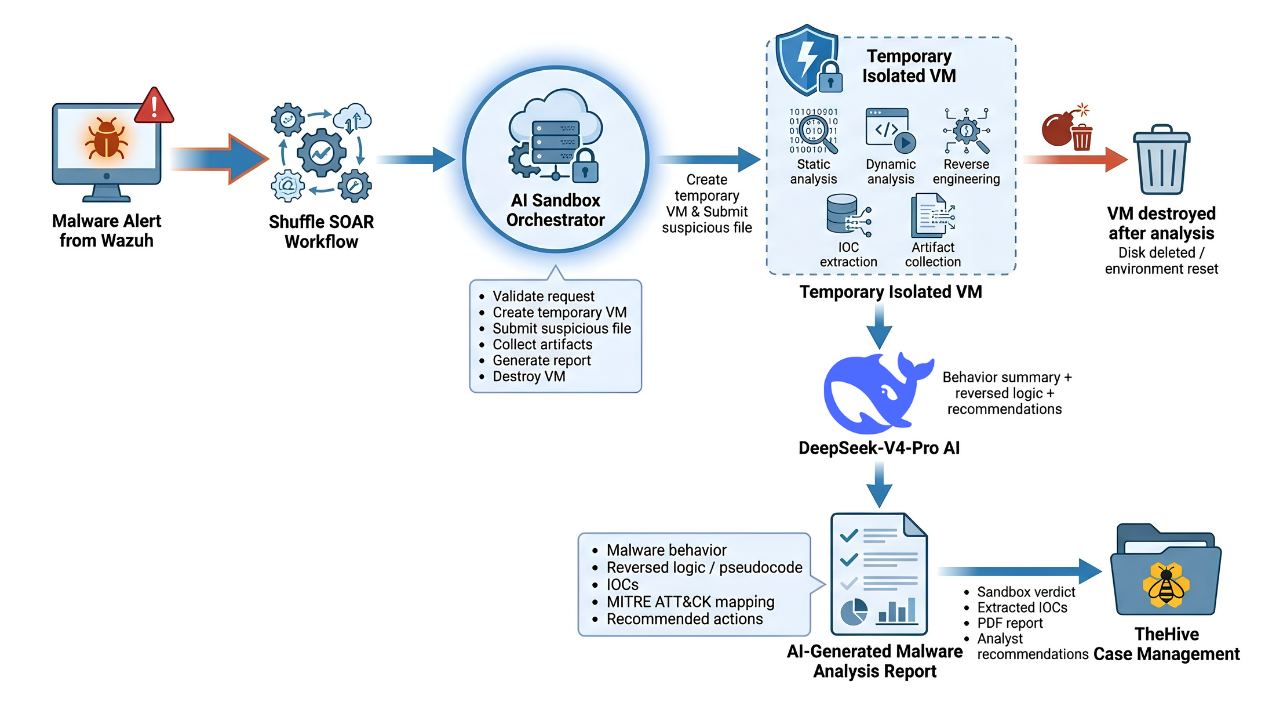
\includegraphics[width=0.82\textwidth]{figs/ai_sandbox_workflow.png}
\caption{AI Sandbox Architecture}
\label{fig:ch4-ai-sandbox-architecture}
\end{figure}

The workflow begins with a Wazuh malware alert forwarded through Shuffle SOAR to the AI Sandbox Orchestrator. The orchestrator creates a temporary isolated VM, submits the suspicious file for analysis, performs static and dynamic analysis, reverses engineer logic, extracts IOCs and artifacts, destroys the analysis VM, and generates a DeepSeek-V4-Pro PDF report with behavior summary, reversed logic, IOCs, MITRE ATT\&CK mapping, verdict, and recommendations, which is sent to TheHive for analyst review.

\begin{figure}[H]
\centering
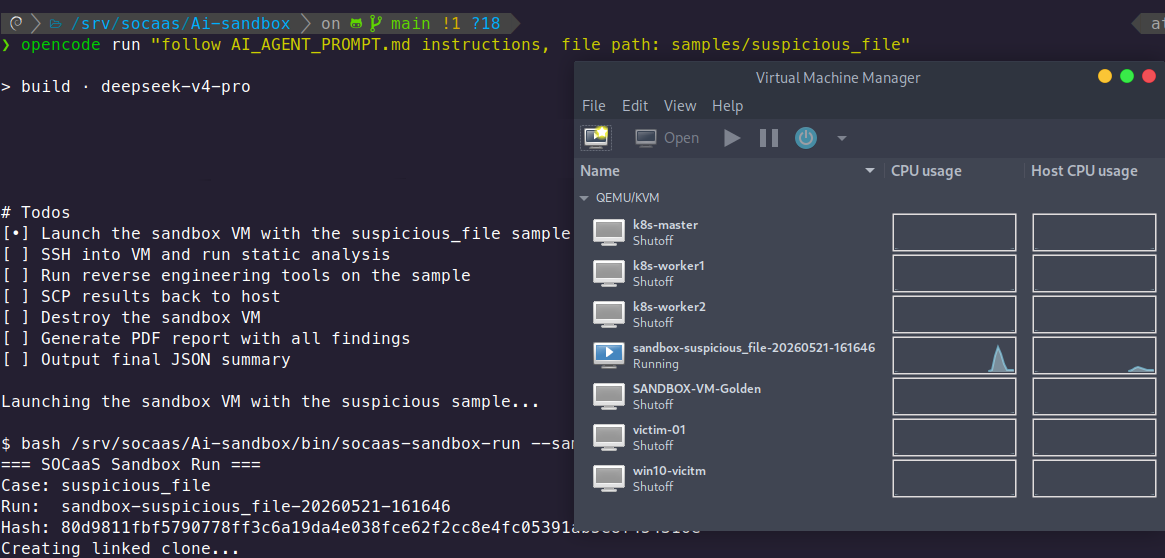
\includegraphics[width=0.82\textwidth]{figs/ai_sandbox_after_opencode_run.png}
\caption{AI Sandbox Orchestrator Request}
\label{fig:ch4-sandbox-request}
\end{figure}

Terminal view showing the sandbox run command issued to the AI Sandbox Orchestrator, displaying the case name \texttt{suspicious\_file}, run ID, and file hash. The Virtual Machine Manager shows the temporary sandbox VM created from the golden image.

% ========== 4.9 AI SANDBOX CASE STUDY: PASSWORD FILE EXFILTRATION SCRIPT ==========
\section{AI Sandbox Case Study: Password File Exfiltration Script}
\label{sec:ch4-ai-sandbox-case-study}

A controlled malware sample was used to validate the AI Sandbox under laboratory conditions. The sample was intentionally developed for the SOCaaS validation environment as a compact Python program whose objective was to search the local filesystem for filenames containing the word \texttt{password}, collect the contents of matching files, and transmit the gathered data to a controlled listener at \texttt{192.168.122.1:4444}. This scenario was selected because it combines several behaviors that are relevant to defensive analysis: recursive discovery, selective file targeting, credential harvesting intent, outbound communication, and structured data exfiltration.

The sample was submitted to the AI Sandbox as a suspicious artifact without giving the AI report-generation stage direct access to the original source code. In other words, the objective of the experiment was not to ask the model to summarize known code, but to determine whether the sandbox workflow could infer the same logic independently from the collected analysis evidence. This distinction is important from a validation perspective, because the generated report must reflect recovered behavior rather than source-level restatement.

For publication safety, the thesis includes a sanitized, non-operational excerpt that preserves the analytical structure of the laboratory sample without reproducing a reusable exfiltration tool. The original validation specimen remained confined to the controlled environment described in this work.

\begin{lstlisting}[style=socaaspython,caption={Sanitized excerpt of the controlled laboratory sample used for AI Sandbox validation},label={lst:ch4-sanitized-lab-sample}]
#!/usr/bin/env python3
import os

TARGET_LABEL = "controlled_listener"

def collect_password_files():
    matches = []
    for root, dirs, files in os.walk("."):
        for filename in files:
            if "password" not in filename.lower():
                continue
            filepath = os.path.join(root, filename)
            try:
                with open(filepath, "r", encoding="utf-8", errors="ignore") as handle:
                    content = handle.read()
            except Exception:
                continue
            matches.append((filepath, content))
    return matches

def prepare_validation_summary(matches):
    # Network transmission intentionally removed for publication safety.
    return [{"path": filepath, "preview_length": len(content)}
            for filepath, content in matches]

def main():
    matches = collect_password_files()
    _ = prepare_validation_summary(matches)

if __name__ == "__main__":
    main()
\end{lstlisting}

Listing~\ref{lst:ch4-sanitized-lab-sample} reflects the logical structure of the controlled validation sample in a sanitized form. The original laboratory sample recursively searched directories for files whose names contained the word \texttt{password}. Matching files were collected and, in the live validation specimen, their contents were prepared for exfiltration through a TCP connection to a controlled listener. The version displayed in the thesis intentionally removes the operational transmission stage while preserving the discovery and collection logic that was relevant to the case study.

The AI Sandbox identified the submitted artifact as a Python-based credential harvester and data exfiltration tool. The generated analysis recovered the same behavioral chain as the original sample: recursive file traversal, filename matching, content collection from targeted files, TCP-based exfiltration behavior, the destination \texttt{192.168.122.1:4444}, and the use of a payload structure carrying both file path and file content. The report further extracted indicators of compromise, including the SHA256 hash of the sample, the destination IP address, TCP port \texttt{4444}, the searched filename pattern containing \texttt{password}, and a network signature consistent with outbound exfiltration activity.

The strongest validation result is that the AI Sandbox reconstructed the same malicious logic and behavior as the original source code. The generated AI report successfully identified recursive file traversal, filename matching, credential harvesting behavior, TCP exfiltration, the destination IP address and port, IOC extraction, and explicit malicious intent. Most importantly, the reversed logic generated by the AI closely matched the original implementation, despite the fact that the analysis stage did not rely on direct access to the source code itself. This demonstrates that the sandbox can recover operationally meaningful malware behavior from analysis artifacts and present it in a form that is immediately usable by analysts.

The report also generated analyst response guidance, including blocking the extracted IOCs, investigating the controlled listener, scoping the affected endpoint, hunting for possible data loss, rotating exposed credentials, preserving forensic evidence, and enforcing policies against plaintext password files. These recommendations demonstrate that the AI Sandbox not only classifies a suspicious file, but also accelerates the next steps of the incident response process.

\begin{figure}[H]
\centering
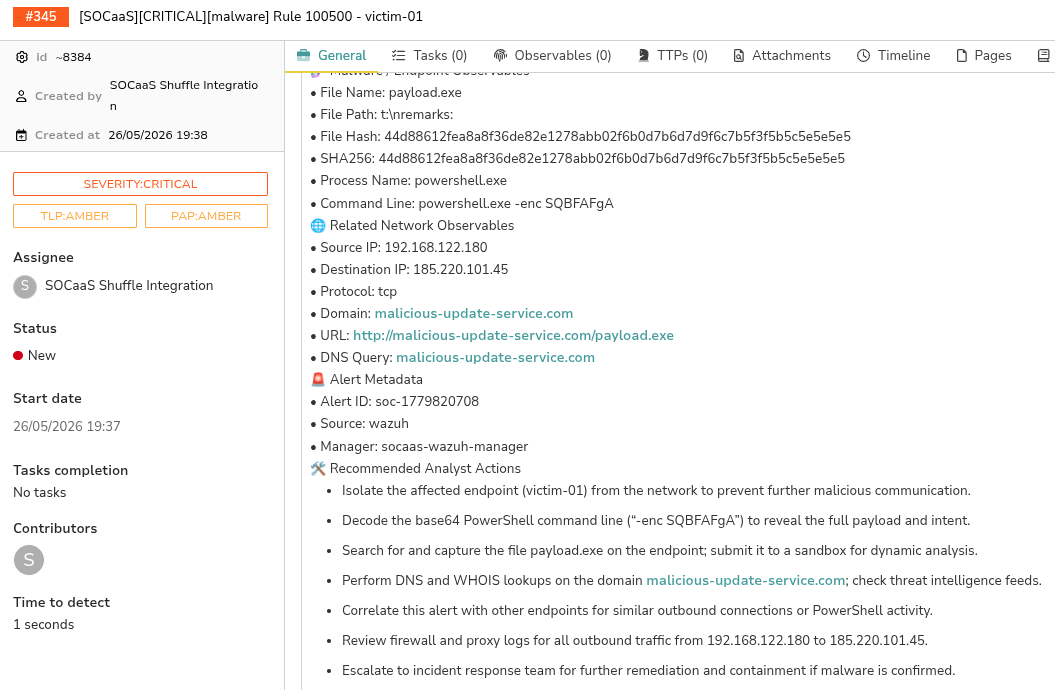
\includegraphics[width=0.95\textwidth]{figs/thehive_malware_case_ai_recommendations.png}
\caption{TheHive Malware Case with AI Recommended Actions}
\label{fig:ch4-thehive-malware-ai-recommendations}
\end{figure}

The TheHive case view preserves the AI-generated response guidance together with the malware alert context, allowing the analyst to review recommendations inside the formal incident record.

The complete AI-generated malware analysis report, including reversed logic, IOC extraction, MITRE ATT\&CK mapping, risk assessment, and recommendations, is provided in Appendix~C (see Appendix~\ref{app:ai-sandbox-report}).

\begin{figure}[H]
\centering
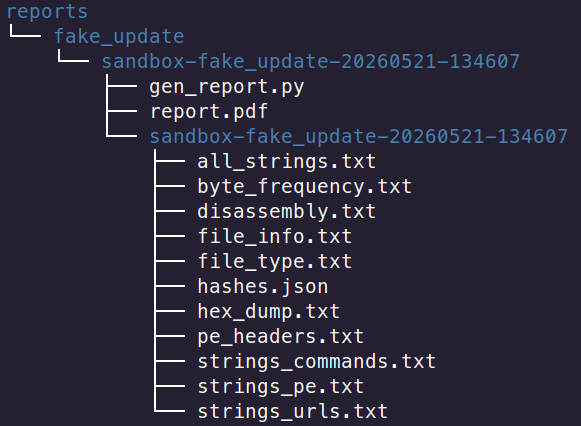
\includegraphics[width=0.82\textwidth]{figs/ai_sandbox_reports_artifacts_tree.png}
\caption{Static Analysis Artifacts}
\label{fig:ch4-static-analysis-summary}
\end{figure}

The directory tree shows the generated analysis output for the controlled sample, including \texttt{report.pdf}, \texttt{hashes.json}, \texttt{strings\_pe.txt}, \texttt{strings\_urls.txt}, \texttt{disassembly.txt}, \texttt{file\_info.txt}, \texttt{pe\_headers.txt}, \texttt{hex\_dump.txt}, \texttt{byte\_frequency.txt}, and other static analysis evidence collected during the sandbox run.

\begin{figure}[H]
\centering
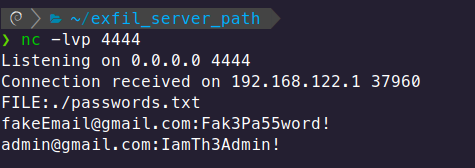
\includegraphics[width=0.82\textwidth]{figs/exfil_server_path_listener.png}
\caption{Observed IOC Behaviour -- Netcat Exfiltration Listener}
\label{fig:ch4-ioc-extraction}
\end{figure}

A netcat listener on port 4444 receives a connection and captures the exfiltrated content \texttt{FILE: ./passwords.txt} along with example credentials, confirming the C2 communication pattern of the controlled sample and providing runtime evidence for IOC extraction.

% ========== 4.10 VALIDATION SCENARIOS ==========
\section{Validation Scenarios}
\label{sec:ch4-validation-scenarios}

Three validation scenarios were used to evaluate SOCaaS. The main scenario is the malware and AI Sandbox validation because it demonstrates the added value of SOCaaS beyond detection and notification. Two additional scenarios were performed to validate reconnaissance and command-and-control detection. The technical commands, screenshots, and detailed evidence for these two scenarios are placed in Appendix A and Appendix B to keep this chapter focused on implementation and analysis.

\subsection{Malware and AI Sandbox Validation}
\label{subsec:ch4-malware-validation}

The malware validation scenario tested whether SOCaaS could support the investigation of a suspicious file. The controlled Python exfiltration sample was submitted to the AI Sandbox. The sandbox performed analysis, extracted indicators, reconstructed behavior, produced a risk verdict, generated recommendations, and created a five-page PDF report.

The validation was successful because the generated report recovered the intended behavior of the original sample. It identified recursive file searching, filename matching for \texttt{password}, file reading, TCP exfiltration, and the destination \texttt{192.168.122.1:4444}. The report also identified relevant IOCs and recommended analyst actions. This result validates the AI Sandbox as a useful SOCaaS capability for first-level malware triage.

From an operational perspective, the scenario shows that SOCaaS can shorten the time required to understand suspicious file behavior. The analyst receives an evidence-based malware report and can immediately focus on containment, scoping, credential rotation, and forensic preservation instead of beginning with manual code analysis.

\begin{figure}[H]
\centering
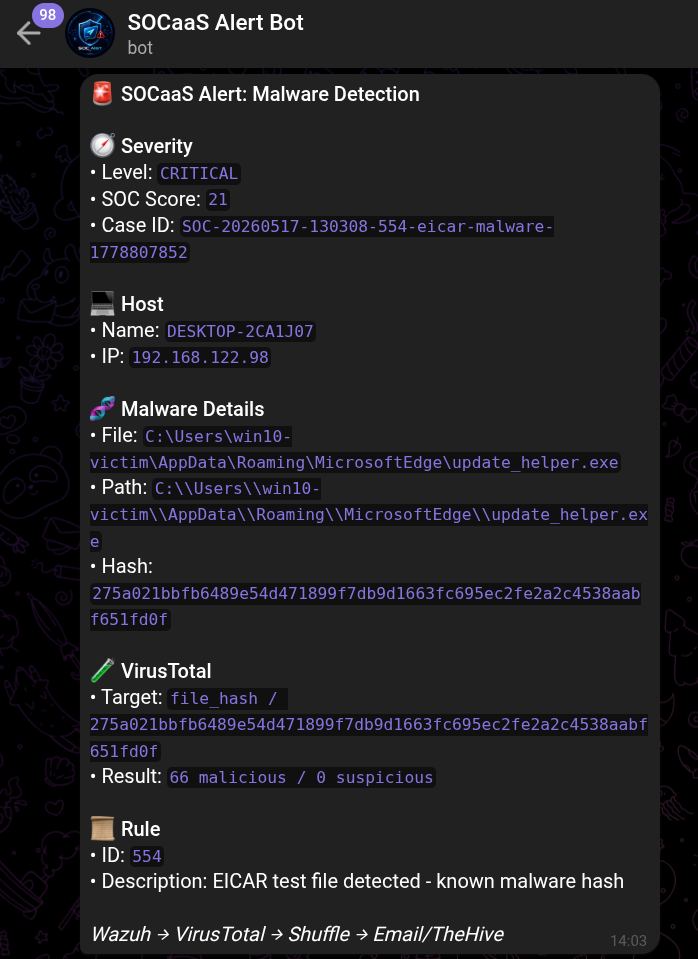
\includegraphics[width=0.55\textwidth]{figs/telegram_malware_notification.png}
\caption{Telegram Notification for Malware Detection}
\label{fig:ch4-telegram-malware-notification}
\end{figure}

The Telegram notification confirms that the malware scenario produced analyst-facing notification evidence while preserving richer investigation context in TheHive and the AI Sandbox report.

\subsection{Nmap Port Scan Validation}
\label{subsec:ch4-nmap-validation}

The Nmap port scan scenario validated reconnaissance detection. A controlled scan was executed against a monitored endpoint. Wazuh generated alerts using the custom port scan and UFW-related detection rules. The Pipeline Gateway received the alerts, extracted relevant observables such as source IP address, destination IP address, and ports, then reduced repeated alerts through the 300-second deduplication cache.

Shuffle processed the normalized alert, sent analyst notifications, and created a case in TheHive. This confirmed that SOCaaS can detect and automate triage for network reconnaissance activity. The detailed Nmap scenario, screenshots, and technical evidence are provided in Appendix A: Nmap Port Scan Detection and Response.

\subsection{C2 Beacon Validation}
\label{subsec:ch4-c2-validation}

The C2 beacon scenario validated command-and-control detection. The test involved suspicious outbound communication from a monitored endpoint toward a controlled listener. Wazuh detected the suspicious activity, and the Pipeline Gateway extracted the relevant IP, port, domain, or process context available in the alert.

The alert was enriched, processed by Shuffle, and supported by AI-assisted recommendations. These recommendations guided analyst actions such as containment of the affected host, blocking of suspicious communication, process investigation, and hunting for related events. The detailed C2 scenario, screenshots, and technical evidence are provided in Appendix B: C2 Beacon Detection and Response.

% ========== 4.11 EVALUATION OF RESULTS ==========
\section{Evaluation of Results}
\label{sec:ch4-evaluation}

The SOCaaS implementation was evaluated according to detection success, forwarding reliability, enrichment quality, deduplication effectiveness, notification delivery, case creation, AI-assisted recommendation usefulness, and AI Sandbox report generation. The results show that SOCaaS successfully connects endpoint monitoring to automated investigation workflows.

\begin{table}[H]
\centering
\caption{Evaluation of SOCaaS Implementation Results}
\label{tab:ch4-evaluation-results}
\renewcommand{\arraystretch}{1.35}
\begin{tabularx}{\textwidth}{>{\RaggedRight\arraybackslash}p{4cm} >{\RaggedRight\arraybackslash}p{2.6cm} X}
\toprule
\rowcolor{tableheader}
\textbf{Evaluation Point} & \textbf{Result} & \textbf{Evidence} \\
\midrule
Wazuh detection & Successful & Alerts were generated from monitored Linux and Windows endpoints. \\
\midrule
Pipeline forwarding & Successful & The \texttt{/hooks/wazuh} endpoint received alerts from the Wazuh Alert Forwarder. \\
\midrule
Deduplication & Successful & Repeated alerts were reduced through the 300-second TTL cache. \\
\midrule
VirusTotal enrichment & Successful & Extracted observables were enriched where reputation lookup was meaningful. \\
\midrule
Shuffle workflow & Successful & The \texttt{SOCaaS Wazuh Alert Triage} workflow completed successfully. \\
\midrule
Telegram notification & Successful & Analysts received short alert notifications. \\
\midrule
Email notification & Successful & Analysts received richer alert context by email. \\
\midrule
TheHive case creation & Successful & Cases were created in the \texttt{socaas} organization. \\
\midrule
AI recommendations & Successful & Structured analyst actions were generated from normalized alert context. \\
\midrule
AI Sandbox report & Successful & A five-page PDF malware analysis report was generated. \\
\midrule
Sandbox logic extraction & Successful & The reconstructed logic matched the original behavior of the controlled sample. \\
\midrule
Analyst time reduction & Positive & The report summarized reverse engineering findings and reduced first-level triage effort. \\
\bottomrule
\end{tabularx}
\end{table}

The results demonstrate that SOCaaS performs more than alert collection. Wazuh detects suspicious behavior, the Pipeline Gateway normalizes and enriches alerts, Shuffle automates response actions, and TheHive stores the investigation context. The AI recommendation node improves the analyst starting point by generating structured response guidance from verified alert data.

The AI Sandbox produced the strongest validation result. It generated a five-page PDF report and reconstructed the behavior of the controlled malware sample. This shows that malware analysis time can be reduced from manual reverse engineering to automated first-level triage and report review. For SMEs, this is an important operational advantage because it provides malware understanding without requiring a dedicated reverse engineering team.

Timing metrics can also be reported when supported by screenshots and workflow evidence. If alert timestamps confirm the result, the Mean Time to Detect can be reported as less than or equal to one minute. If the workflow execution evidence supports it, the Mean Time to Respond can be discussed around fifteen minutes. These measurements should be documented using the available screenshots and execution records rather than estimated without evidence.

% ========== 4.12 LIMITATIONS AND SECURITY CONSIDERATIONS ==========
\section{Limitations and Security Considerations}
\label{sec:ch4-limitations}

Although the SOCaaS implementation successfully validates the proposed platform, several limitations and security considerations must be acknowledged. The Kubernetes cluster uses a single control-plane node. This is acceptable for the laboratory implementation, but it does not provide Kubernetes control-plane high availability. A production deployment should use multiple control-plane nodes and appropriate backup procedures \cite{k8s-docs,luksa2017kubernetes}.

AI-assisted recommendations require analyst validation. The AI component improves triage and report readability, but it does not replace deterministic detection, verified evidence, or human decision-making. Analysts remain responsible for confirming incident scope, approving containment actions, and validating the relevance of recommendations.

The AI Sandbox must remain isolated. Suspicious files should be analyzed only inside a temporary isolated VM, and infected virtual machines must not be reused. The implemented lifecycle, in which the temporary VM is destroyed after analysis and its disk is deleted, reduces contamination risk and supports safer malware handling \cite{sikorski2012malware,nist-sp800-83r1}.

Malware sample acquisition must also be controlled. Samples should be collected, stored, transferred, and analyzed only under authorized conditions. The thesis does not reproduce full malware source code or provide dangerous step-by-step malware-building instructions. The controlled exfiltration sample is discussed only through its observed behavior and generated report findings.

Threat intelligence enrichment must be interpreted carefully. Private IP addresses from the laboratory network, such as addresses in \texttt{192.168.122.0/24}, cannot be meaningfully scored by public reputation services. In such cases, internal context and endpoint evidence are more important than external reputation scores.

For production use, SOCaaS should enforce TLS for exposed services, strengthen secrets management, improve access control, and persist deduplication state where operationally required. The AI Sandbox report should support expert analysis rather than replace it, especially during high-impact incidents or cases requiring forensic-grade conclusions.

% ========== 4.13 CONCLUSION ==========
\section{Conclusion}
\label{sec:ch4-conclusion}

This chapter presented the implementation and validation of the SOCaaS platform. The platform was deployed as an open-source, cloud-native SOC on Kubernetes using one control-plane node and two worker nodes. Wazuh provided endpoint detection, the Pipeline Gateway performed normalization, enrichment, and deduplication, Shuffle SOAR automated the incident response workflow, and TheHive provided case management.

The validation scenarios showed that SOCaaS can detect suspicious activity, process alerts, notify analysts, create cases, and enrich investigations with AI-assisted recommendations. The Nmap and C2 scenarios validated reconnaissance and command-and-control detection and are documented in detail in Appendix A and Appendix B.

The main contribution of this chapter is the AI Sandbox. SOCaaS does not only detect and notify; it accelerates investigation by producing an AI-generated malware analysis report containing reconstructed logic, IOCs, MITRE ATT\&CK mapping, a risk verdict, and recommended analyst actions. The controlled password-file exfiltration sample demonstrated that the AI Sandbox could recover the same behavior as the original script and produce a five-page report suitable for analyst triage.

The supporting evidence is organized as follows: Appendix A presents Nmap Port Scan Detection and Response, Appendix B presents C2 Beacon Detection and Response, and Appendix C provides the AI Sandbox Generated Malware Analysis Report.
